% This is samplepaper.tex, a sample chapter demonstrating the
% LLNCS macro package for Springer Computer Science proceedings;
% Version 2.20 of 2017/10/04
%

\documentclass[runningheads]{llncs}

\usepackage{times}
\usepackage{ifpdf}
\usepackage[english]{babel}
\usepackage{cite}
\usepackage[utf8]{inputenc}

\usepackage{graphicx}
\usepackage{amssymb,amsmath,amsfonts} 
\usepackage{balance}

\usepackage{color}
\usepackage{hyperref}
\usepackage[nocenter]{qtree}
\usepackage{tree-dvips}
\usepackage{listings}

\definecolor{lightgrey}{rgb}{0.95,0.95,0.95}

\newcommand{\IS}		{INScore}
\newcommand{\exemple}	{\vspace*{1mm}\hspace*{-4mm}\textbf{Example :}}

\definecolor{mygrey}{gray}{0.93}
\newcommand{\code}	[2][0.9]	{\vspace{0mm}\begin{center}\colorbox{mygrey}{
							\begin{minipage}[t]{#1\columnwidth} 
							{\small \texttt{#2}}
							\end{minipage}}\end{center}}

\newcommand{\op}	[1]		{\vspace{0mm}\begin{center}\colorbox{mygrey}{
							\begin{minipage}[t]{0.9\columnwidth} 
							{\small \texttt{#1}}
							\end{minipage}}\end{center}}
\newcommand{\llist}	[1]		{\ensuremath{[#1_1,...,#1_k]}}

\newcommand{\nulltree}	{\ensuremath{\varnothing}}
\newcommand{\seq}		{\ensuremath{|}}
\newcommand{\paral}		{\ensuremath{\parallel}}
\newcommand{\foret}		{\ensuremath{F}}
\newcommand{\toforet}	{\ensuremath{\mathcal{F}}}
\newcommand{\expand}	{\ensuremath{\rightsquigarrow}}
\newcommand{\transform}	{\ensuremath{\xi}}
\newcommand{\binop}		{\ensuremath{op}}
\newcommand{\logop}		{$lop$}
\newcommand{\ftree}		{ftree}
\newcommand{\etc}		{\ensuremath{…}}

\newcommand{\nexpand}	{\ensuremath{\varepsilon}}
\newcommand{\ula}		{\hspace*{8mm}}
\newcommand{\ulb}		{\hspace*{4mm}}
\newcommand{\ulc}		{\hspace*{37mm}}
\newcommand{\uld}		{\hspace*{9mm}}
\newcommand{\ule}		{\hspace*{31.5mm}}
\newcommand{\ulf}		{\hspace*{39mm}}


% ====================================================
\hypersetup{
    colorlinks,%
    citecolor=black,%
    filecolor=black,%
    linkcolor=black,%
    urlcolor=black
}


% ====================================================
\begin{document}

\title{A Tree Based Language for Music Score Description.}

\author{D. Fober\inst{1} \and
Y. Orlarey\inst{1} \and
S. Letz\inst{1} \and R. Michon\inst{1}}
%
\authorrunning{Fober et al.}
% First names are abbreviated in the running head.
% If there are more than two authors, 'et al.' is used.
%
\institute{Grame-CNCM  Lyon - France \\ 
\email{\{fober,orlarey,letz,michon\}@grame.fr}}


\maketitle

%
\begin{abstract}
The presented work is part of the \IS\ project, an environment for the design of augmented interactive music scores, oriented towards unconventional uses of music notation and representation, including real-time symbolic notation capabilities. This environment is fully controllable using Open Sound Control [OSC] messages. \IS\ scripting language is an extended textual version of OSC messages that allows you to design scores in a modular and incremental way. This article presents a major revision of this scripting language, based on the description and manipulation of trees.

\keywords{Music notation \and Language \and INScore.}
\end{abstract}
%

%-------------------------------------------------
\section{Introduction}\label{sec:introduction}

There is a large number of musical score description languages (Lilypond \cite{lilypond03}, Guido \cite{hoos98}, MuseData \cite{Hewlett97}, MEI \cite{Roland_2002}, MusicXML \cite{good01} etc.) that are all turned towards common western music notation. 
The extension of some of these languages has been considered, in order to add \textit{programmability} e.g. operations to compose musical scores in Guido \cite{fober12b}, or the Scheme language in Lilypond.
There are also programming languages dedicated to music notation, like CMN \cite{Schottstaedt97} or ENP 
\cite{KUUSK06} which are in fact Lisp dialects, still oriented towards the common western notation.

The approach proposed by \IS\ \cite{Fober:12a} is quite radically different: symbolic music notation is supported (via the Guido language and rendering engine \cite{Dau:09b,hoos98}), but it constitutes one of the means of music representation among others, without being privileged. 
Purely graphic scores can be designed, but all the elements of a score have a temporal dimension (date, duration and tempo) and can be manipulated both in the graphic and time space. In a way that is somewhat similar to Antescofo \cite{acont08}, the notion of time is both event-driven and continuous \cite{fober17c}, which makes it possible to design interactive and dynamic scores. Figure \ref{pavlos} presents an example of a score realised using \IS . It includes symbolic notation, pictures, a video, and cursors (the video is one of them) which position is synchronised by the performer gestures.

\begin{figure}
\begin{center}
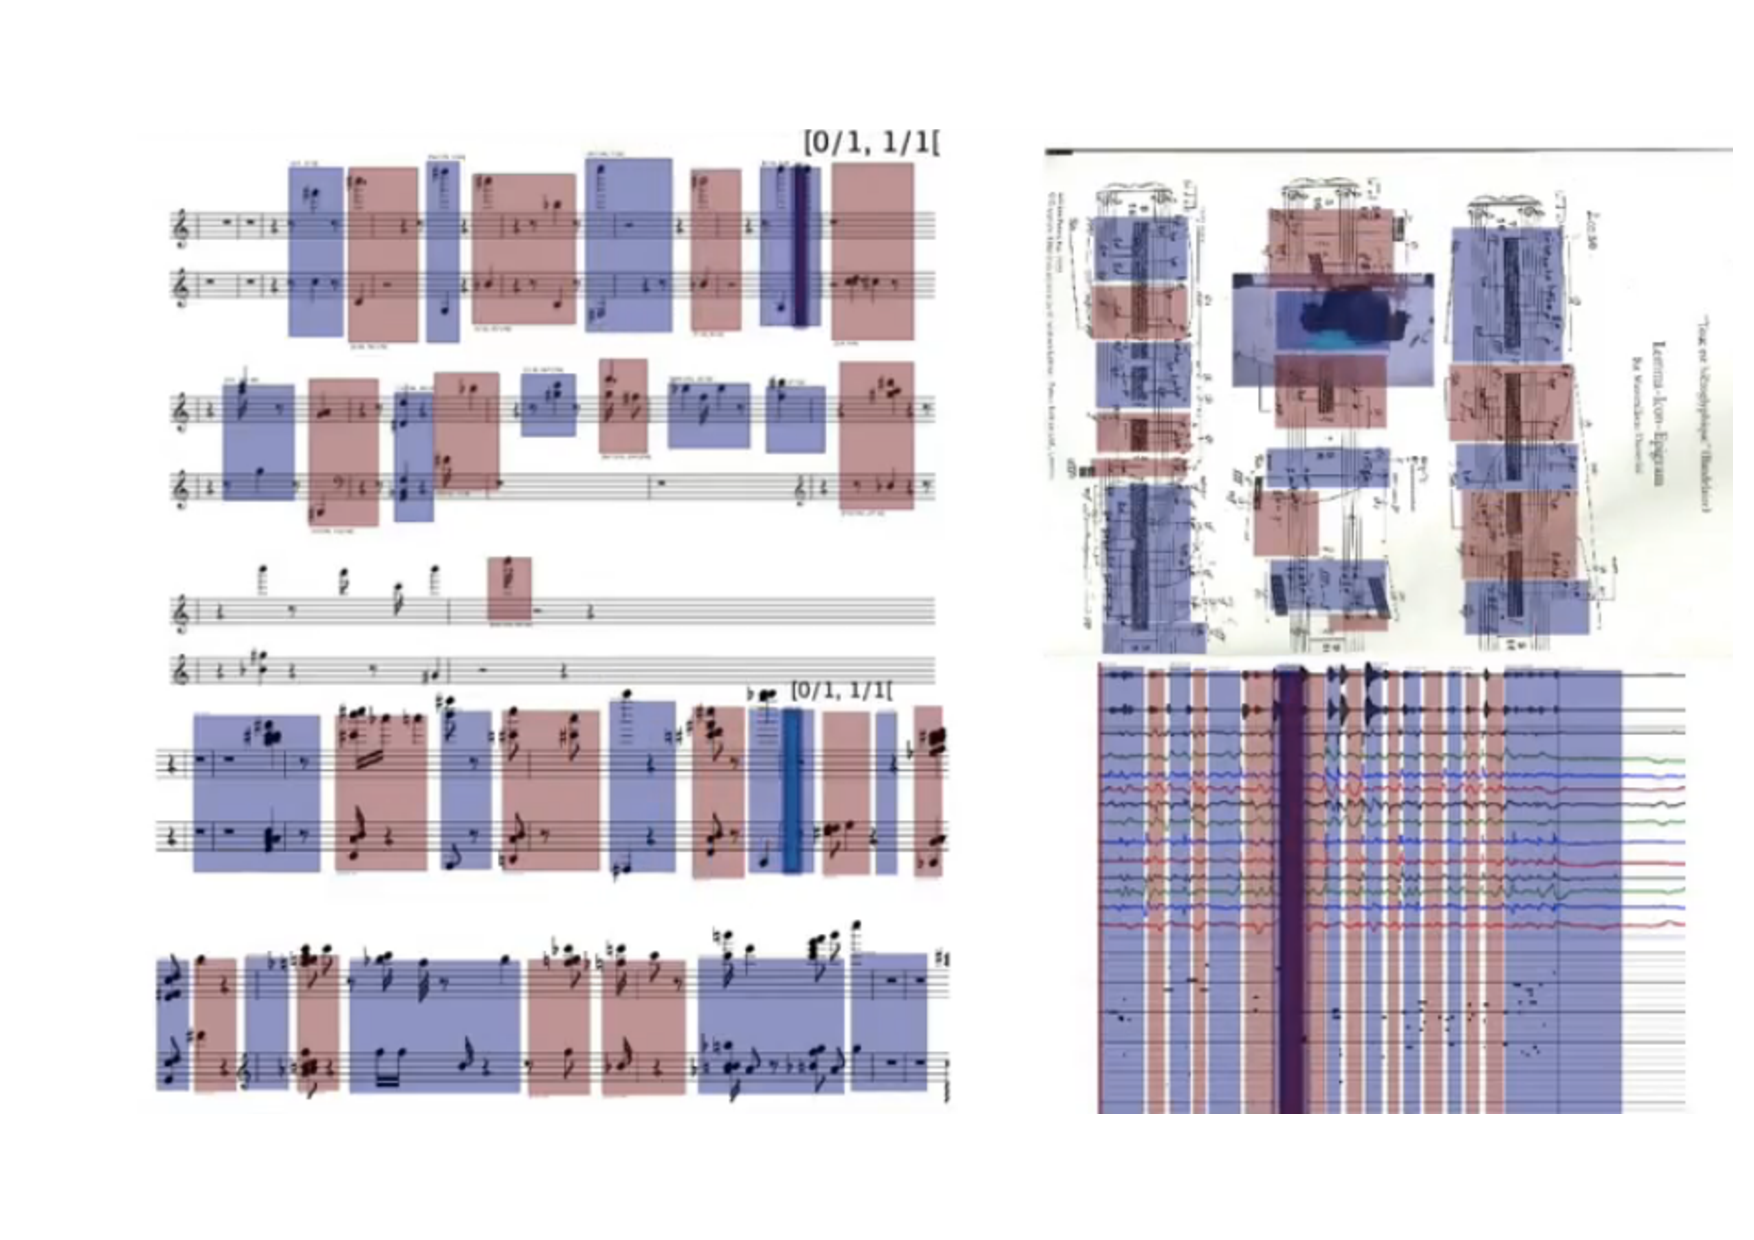
\includegraphics[width=0.75\columnwidth]{imgs/inscore-score}
\caption{A score realised using \IS , used as part of a sensor-based environment for the processing of complex music called \emph{GesTCom} (\emph{Gesture Cutting through Textual Complexity}) \cite{antoniadis:tel-01861171}.}
\label{pavlos}
\end{center}
\end{figure}

\IS\ has been initially designed to be driven by OSC messages \cite{OSC}. OSC is basically a communication protocol. Recently, programming capabilities have been added \cite{429}, in the form of \emph{functions} embedded in OSC messages, allowing structured functional communication between musical applications \cite{bresson:hal-01353794}. 
A textual version of the \IS\ OSC messages constitutes \IS\ storage format, which has been extended to a scripting language, \cite{Fober:13b} allowing greater flexibility in music scores design.
These extensions (introduction of variables, extended addresses, Javascript section, etc.) have nevertheless suffered from a rigidity inherent to an ad hoc and incremental design. For example, the parser makes a clear distinction between OSC addresses and associated data, which prevent the use of variables (at least as currently defined) in OSC addresses.

As a result, a major revision of this language became necessary. It is based on the manipulation of a regular tree structure which is also homogeneous to the \IS\ model.
Figure \ref{tree1} gives an example of such hierarchy, which can be described in the current scripting language (i.e. OSC) by listing all branches from the root. % (Figure~\ref{script1})

\vspace{-4mm}

\begin{figure}
\begin{center}
\Tree [ .ITL [ .scene 
	[ .obj1 [ .x 0 ] [ .y 0 ] [ .date 0 ] ] 
	[ .obj2 [ .x 0.5 ] [ .y 0.5 ] [ .date 1 ] ] ] 
]
\caption{A score sample including 2 objects $obj1$ and $obj2$, having a $x$, $y$, and $date$ attributes. The leaves of the tree are the values of the attributes. Time properties (date, duration) are notably used to represent the time relationship between objects }
\label{tree1}
\end{center}
\end{figure}

After some definitions, we will present the basic operations on trees and the corresponding grammar. We will then introduce mathematical operations on trees, the concepts of \emph{variables} and \emph{nodes in intention} and we'll present how this language is turned into OSC messages. The final section gives an example of the new language before concluding.


%-------------------------------------------------
\section{Definitions}

A tree is a data structure made up of nodes and edges without having any cycle. The tree with no nodes is called the null or empty tree. A tree that is not empty consists of a root node and potentially many levels of additional nodes that form a hierarchy.


%---------------------------
\subsection{Terminology}

\begin{description}
 \setlength\itemsep{0.0em}
\item[Root]	The top node in a tree.
\item[Child]	A node directly connected to another node when moving away from the root.
\item[Parent]	The converse notion of a child.
\item[Leaf]	A node with no children.
\item[Edge]	The connection between one node and another.
\item[Path]	A sequence of nodes and edges connecting a node with a descendant.
\item[Forest]	A list of $n >= 0$ trees.
\end{description}

%---------------------------
\subsection{Trees}
A tree $t$ consists of a value $v$ (of some data type, possibly empty) and a forest $f$ (the subtrees of its children).
\[
	t :  v f \land f = \llist{t} 
\]


%-------------------------------------------------
\section{Operations on Trees}

We define two abstract operations on trees: sequencing and paralleling. These operations have no musical semantics, neither from a temporal nor from a graphic point of view. They are defined as methods for algorithmic construction of OSC messages and operate on the topological organisation of the trees. 

%-----------------------------
\subsection{Putting Trees in Sequence}
Putting two trees $t$ and $t'$ in sequence adds $t'$ as child of all the leaves of $t$.


We will note \seq\ the sequencing operation.
Let 2 trees $t$ and $t'$ be defined as follows:
$t \ :  v \ \ f \ \land f = \llist{t} \\
t' :  v' f'\\$
then
\[
	t \seq\ t'  \to  t" : v\ f" \land f" = [t_1 \seq\ t',\etc, t_k \seq\ t']
\]
with: 
\[
\left\{
\begin{array}{l}
	t :  v \ [\ \nulltree\ ] \\
	t \seq\ t'  \to  t" : v\ [ t' ] \\
\end{array}
\right.
\]
where \nulltree\ is an empty forest.

The right arrow ($\to$) indicates the result of an expression evaluation.

%-----------------------------
\subsection{Putting Trees in Parallel}
Putting two trees $t$ and $t'$ in parallel consists in putting them in a forest.
We will note \paral\ the parallelisation operation. 
Let 2 trees $t$ and $t'$:
\[
	t \paral\ t'  \to  t" : \foret\ [ t, t' ]
\]
$t"$ is a tree which value \foret\ denotes a forest. 
We'll name \emph{\ftree} the type of tree whose value is \foret\ and we extend the sequencing operation to \emph{\ftree}\ as follows:
\[
\left\{
\begin{array}{l}
	t \ :  v\ [ \nulltree\ ] \\
	t' :  \foret\ f\\
	t \seq\ t'  \to  t" : v f \\
\end{array}
\right.
\]

Parallelisation applied to a \emph{\ftree} is propagated to children. For a tree $t : \foret\ \llist{t}$ and $t' :  v f$ :
\[
\left\{
\begin{array}{l}
	t\  \paral\ t'  \to  t" : \foret\ [t_1,\etc,t_k,t']\\
	t' \paral\ t \ \to  t" : \foret\ [t',t_1,\etc,t_k]\\
\end{array}
\right.
\]


%-------------------------------------------------
\section{Grammar}\label{agram}

A tree is syntactically defined in BNF as follows:
\code{tree := value      \hspace*{8mm} $\to$ t : value [ \nulltree ] \\
\ula | tree tree         \hspace*{4mm} $\to$ t : tree \seq\ tree \\
\ula | / tree            \hspace*{9.7mm} $\to$ t : '/' \seq\ tree\\
\ula | tree , tree       \hspace*{0mm}  $\to$ t : tree \paral\ tree \\
\ula | ( tree )          \hspace*{6mm} $\to$ t : tree \\
\ula ;
}
The right arrow ($\to$) indicates the tree built for each syntactical construct. 
The tree whose value is \emph{slash} (/) plays a special role in the tree conversion to OSC messages. This role is described in section \ref{ssec:slash}.


%-------------------------------------------------
\section{Values and Evaluation}\label{sec:valeurs}

A tree may contain literal values (i.e., text, number) or special values that are among the following types:
\begin{itemize}
 \setlength\itemsep{0.0em}
\item mathematical operators
\item variables
\item node in intention
\item slash (/)
\end{itemize}



%---------------------------
\subsection{Mathematical Operators}

Mathematical operations on trees are seen as operations on their values that preserve the subtrees. These operations include:
\begin{itemize}
% \setlength\itemsep{0.0em}
\item arithmetic operations (+ - * / \%)
\item logical operations ($==$ $<$ $\leq$ $>$ $\geq$)
\item trigonometric functions (sin, cos, tan, asin, acos, atan)
\item hyperbolic functions (sinh, cosh, tanh, asinh, acosh, atanh)
\item exponential and logarithmic functions (exp, log, log10, log2)
\item power and square root (pow, sqrt, cbrt)
\item miscellaneous  (min, max, rand)
\end{itemize}

We will designate these operations by \binop. Then for 2 trees $t : v\ \llist{t}$ and $t' : v'\ \llist{t'}$:
\[
	\binop\ t\ t'  \to  t":  (\binop\ v\ v') [ t_1,\etc,t_k,t'_1,\etc,t'_k ]
\]

%---------------------------
\subsection{Variables}

A variable is the association of an identifier and a tree. Its general form is
$varname = t$.
Evaluation of a variable consists in expanding the corresponding tree at the variable position.
Let a variable $var$ be defined as a tree $t : v f$.
Let then define a tree $t' : \$var f'$.
\emph{\$var} denotes the value of the variable named \emph{var}. The evaluation of $t'$ is defined as:
\[
	t'_{\{var\}}  \to t" : t \seq\ \toforet(t')
\]
where
\[
	\toforet(t : v\ f)  \to t' : \foret\ f
\]

t'$_{\{var\}}$ denotes a tree whose environment contains the definition of the variable $var$. The \toforet\ operation transforms a tree into an \emph{\ftree}.


\exemple
\code{x = x 0;\\
y = y 0;\\
/A/B \$x, \$y; \ \ $\Rightarrow$  /A/B (x 0), (y 1);}


%---------------------------
\subsubsection{Local Environnements}

Each tree is evaluated in an environment containing the list of all the variables of its parent. However, a variable can be evaluated in a local environment, which is defined inside braces:
\[
\left\{
\begin{array}{l}
	var = t \\
	\$var\{a=t1, b=t2,\etc\} \ \to  t' := t_{\{a, b,\etc\}} \\
\end{array}
\right.
\]


%---------------------------
\subsection{Nodes in Intention}

A \emph{node in intention} is a compact description of a forest. It can also be seen as a \emph{loop} control structure. The general form is as follows:
\begin{description}
 \setlength\itemsep{0.0em}
\item $id[n…m]$ 	where $n$ and $m$ are integers
\item $id[ab…xy]$ where $a,b,x,y$ are letters.
\end{description}

Expanding a node in intention transforms that node into a forest. We will note \nexpand\ the expansion operation:
\[
\left\{
\begin{array}{l}
	\nexpand(id[n…m])   \ \ \to \foret \ [id_n,id_{n+1},…,id_m] \\
	\nexpand(id[ab…xy]) \to \foret \ [id_{ab},id_{ac},…,id_{ay}, \\
	\ule id_{bb},id_{bc},…,id_{by},\\
	\ule …,\\
	\ule id_{xb},id_{xc},…,id_{xy}]
\end{array}
\right.
\]

%---------------------------
\subsubsection{Special Forms}

A \emph{node in intention} can take the following special forms: 
\begin{description}
\item $id[i:n…m]$ 	where $i$ is an identifier
\item $id[i:j:ab…xy]$ where $i,j$ are identifiers.
\end{description}
These identifiers denote variables that are instantiated in the environment by the expansion operation, with the current index value. For example for the first form:
\[
	\nexpand(id[i:n…m])   \qquad \to \foret \ [id_{n\{i=0\}},id_{n+1\{i=1\}},…,id_{m\{i=m-n\}}] \\
\]

%---------------------------
\subsection{Slash (/)}\label{ssec:slash}

The \emph{slash} nodes are used to transform a tree into OSC messages. Their purpose is to discriminate the OSC address and the parameters of the message. Transforming a tree into OSC messages consists in enumerating all the paths from the root node up to the first parameter, which is the first node that is not preceded by a \emph{slash}.



%-------------------------------------------------
\section{Example}\label{example}

The script below presents an example of the new version of the \IS\ scripting language. Variables are indicated in blue. Local variables are declared in red.

\lstdefinelanguage{inscore} 
{
classoffset=0,
morekeywords={}, keywordstyle=\color{blue},
classoffset=1,
morekeywords={addr, count, radius, size, pos, color }, keywordstyle=\color{red},
classoffset=2,
keywordsprefix=$,
sensitive=true,
morecomment=[l]{\#},
morestring=[b]", 
}

\lstset{backgroundcolor=\color{lightgrey}, extendedchars=true, inputencoding=utf8}

\begin{lstlisting}[language=inscore, extendedchars=true, basicstyle=\small\ttfamily]
# variables declaration 
pi    = 3.141592653589793;

# '$step' makes use of 'count' a local variable 
step  = / ( * 2, $pi), $count;

# '$i' is defined by the expansion of the address 'n_[i:1...9]'
x = math.sin ( * $step, $i );
y = math.cos ( * $step, $i );

# the following variables select part of guido
# music notation code to build a short score
dyn = (? (% $i, 3), '\i<"p">', '\i<"ff">');
note = (+ $dyn, " ", (?  (% $i, 2), "e2", "g1/8"));

# this is a classical OSC message that simply clears the scene
/ITL/scene/* del;

# this is the main variable. It will be expanded to create 
# a series of small scores. The variables are computed 
# using locally defined variables.  
notes = (/ITL/scene/$addr  
	(set gmn (+ "[", $note, "]")),
	(scale 0.7),
	(x * $x, $radius),
	(y * $y, $radius)); 

# finally '$notes' is used  with addr, count and radius as local
# variables, which could be viewed as a function call.
$notes{addr=n_[i:1...9], count=9, radius=0.7};
\end{lstlisting}


Evaluation of this script produces OSC messages fully compatible with the previous version of the language, and which are schematically presented below. 
\code[1]{/ITL/scene/n\_1 set gmn '[ \i<"ff"> g1/8]';\\
/ITL/scene/n\_1 scale 0.7;\\
/ITL/scene/n\_1 x 0.0;\\
/ITL/scene/n\_1 y 0.7;\\
...\\
/ITL/scene/n\_9 set gmn '[ \i<"ff"> c2]';\\
/ITL/scene/n\_9 scale 0.7;\\
/ITL/scene/n\_9 x -0.411452;\\
/ITL/scene/n\_9 y 0.56631;
}

In practice, this example expresses the scene illustrated by the Figure \ref{samplescene} in just a few lines.  

\begin{figure}[htbp]
\begin{center}
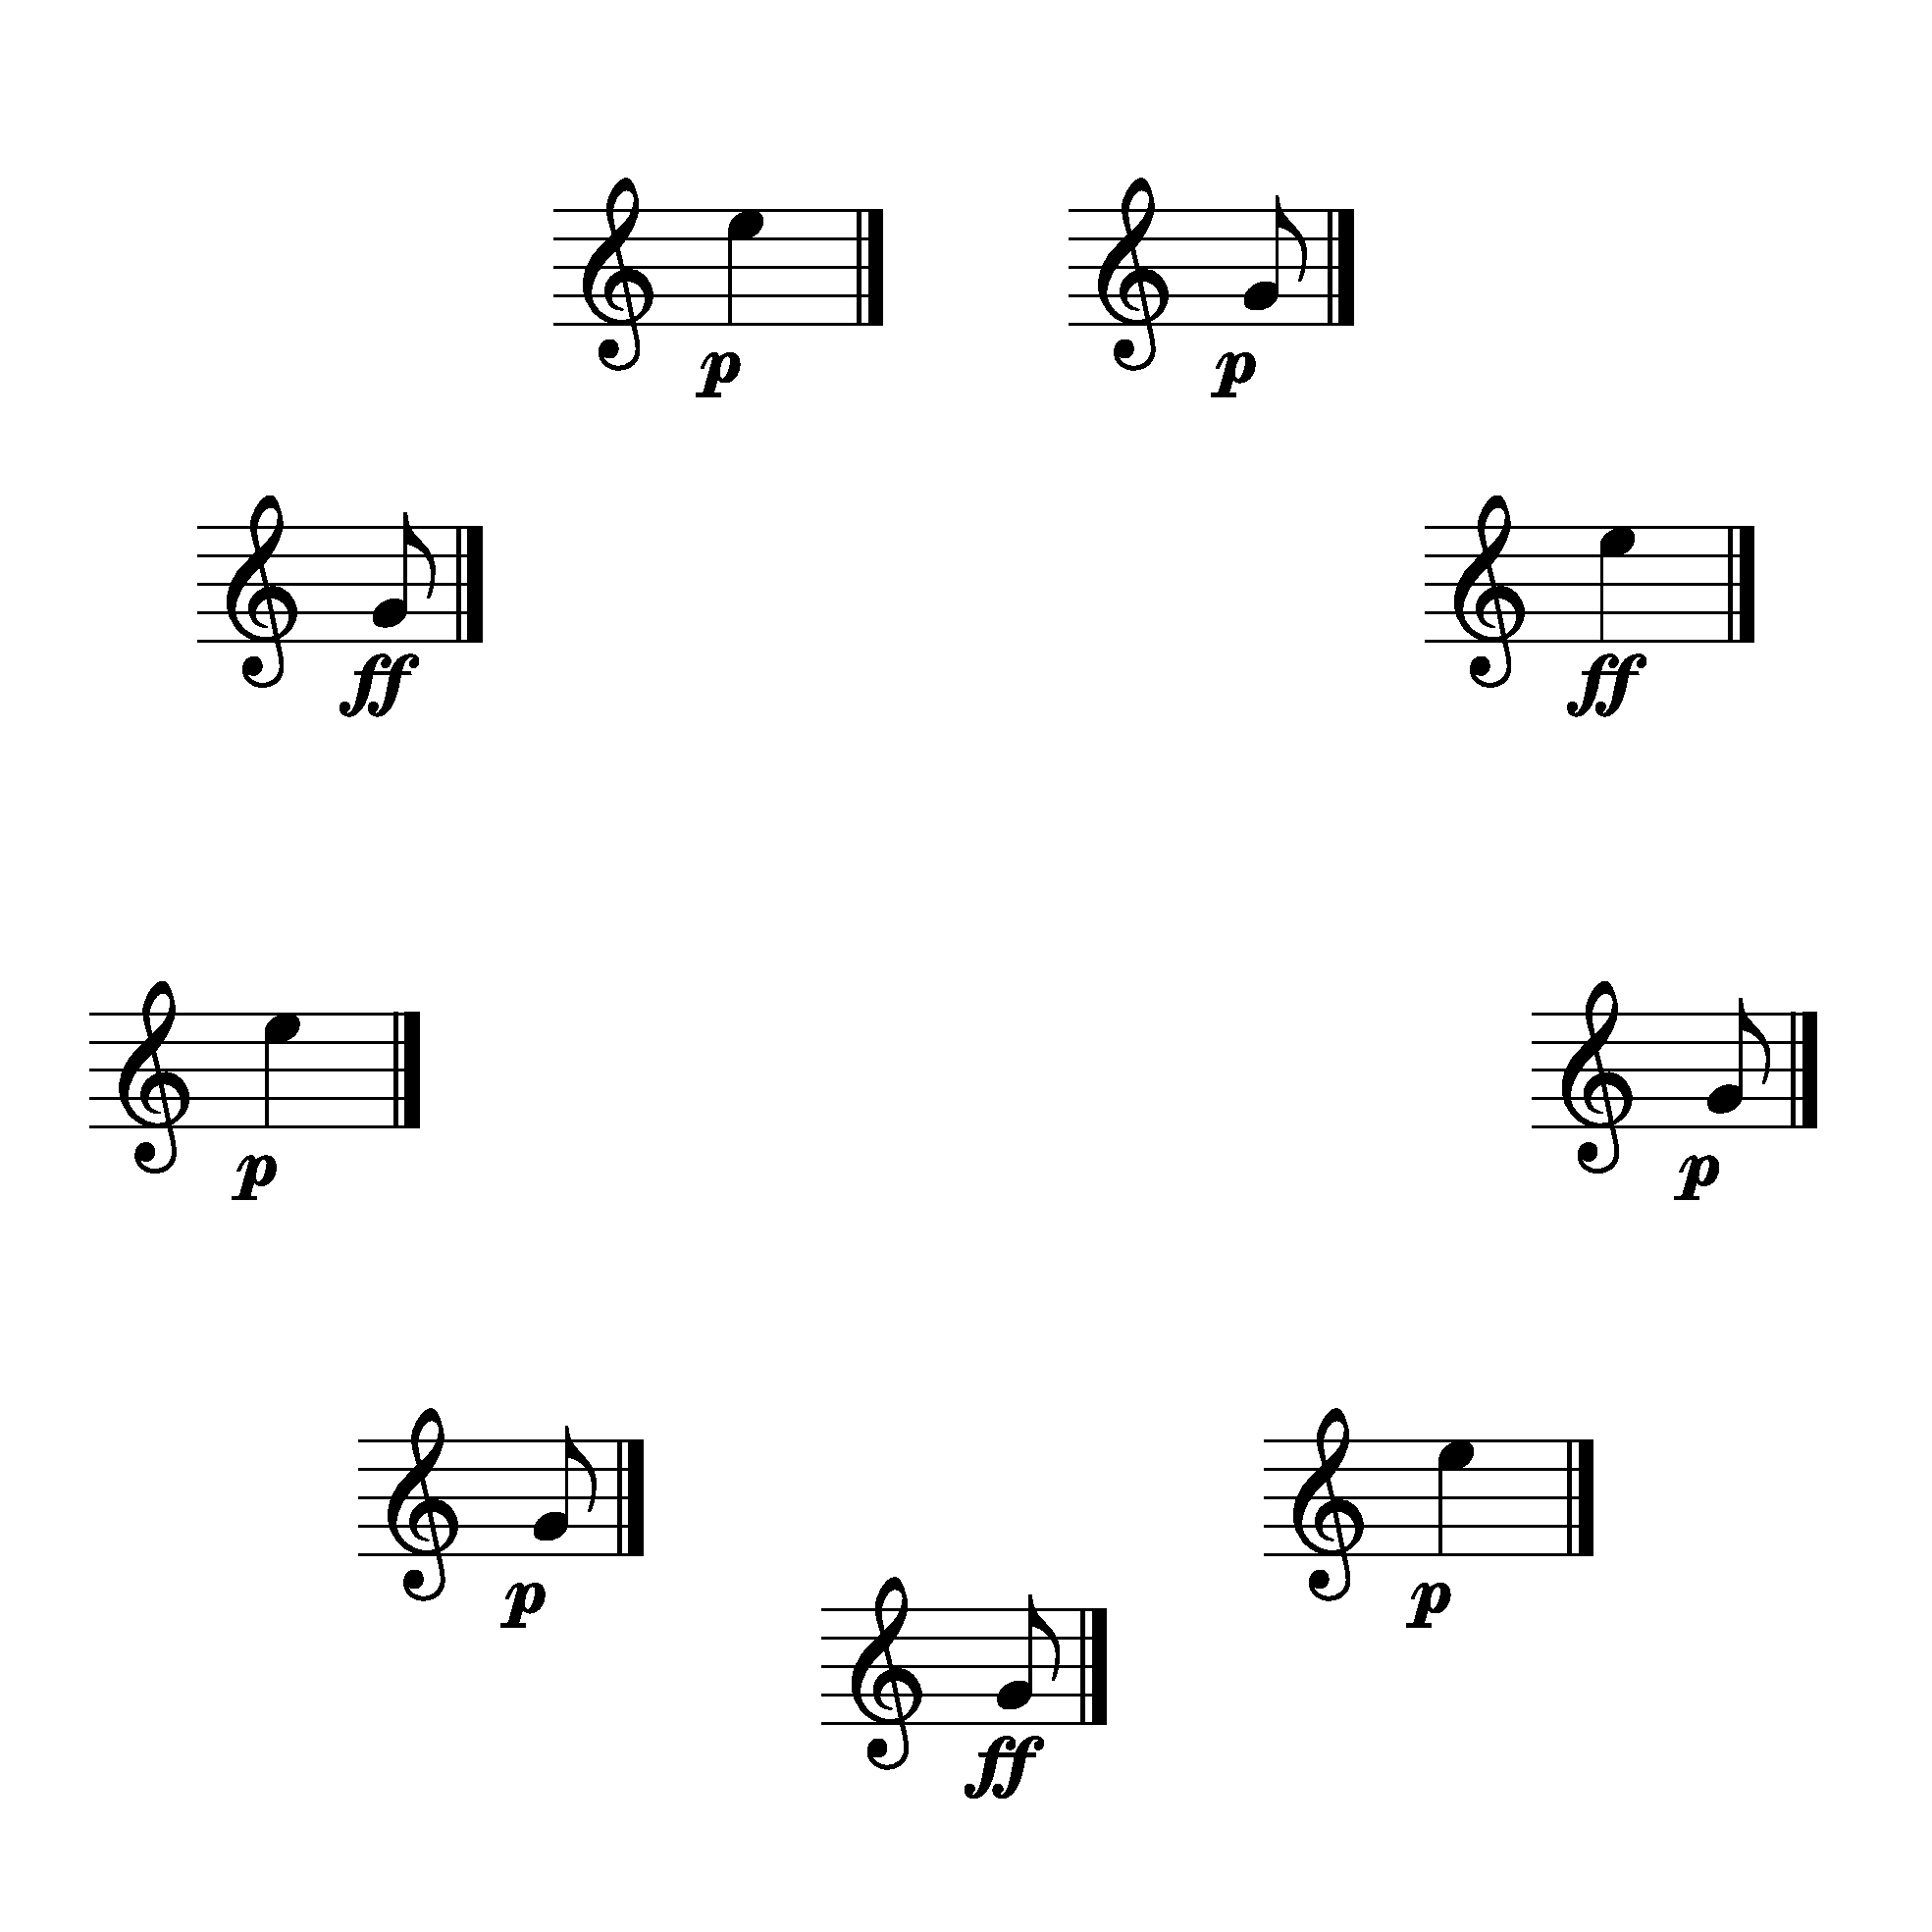
\includegraphics[width=0.65\columnwidth]{imgs/scene}
\caption{\IS\ scene corresponding to the sample script given in section \ref{example}.}
\label{samplescene}
\end{center}
\end{figure}


%-------------------------------------------------
\section{Conclusions}
From two elementary operations on trees - sequencing and parallelisation - we have homogeneously introduced the notions of variables and of mathematical and logical operations on trees. The resulting language is much more expressive and more flexible than the  previous version of the \IS\ scripting language. 
It supports parallelisation of the arguments of a message, variables to describe addresses, series of addresses expressed in a concise manner, use of local variables allowing reusing scripts or parts of scripts in different contexts.



%%%%%%%%%%%%%%%%%%%%%%%%%%%%%%%%%%%%%%%%%%%%%%%%%%%%%%%%%%%%%%%%%%%%%%%%%%%%%
%bibliography here
\balance
\bibliographystyle{splncs04}
\bibliography{../interlude}

\end{document}
